\documentclass[11pt,letterpaper]{article}

\usepackage{mathpazo,fancyhdr,graphicx,wrapfig,color,sidecap,colortbl,bm,cite,sidecap}

\usepackage[labelfont=bf,small]{caption}
 \usepackage{booktabs}
 
\usepackage{subcaption}
 \usepackage[english]{babel}
 
 \usepackage{algorithm}
\usepackage{algpseudocode}
 
 
\definecolor{Red}{rgb}{0.6,0.1,0.2}

 \usepackage{tikz}
\newcommand*\circled[1]{\tikz[baseline=(char.base)]{
            \node[shape=circle,draw,inner sep=1.5pt] (char) {#1};}}
            
            
\renewcommand{\refname}{References cited}

\setlength{\belowcaptionskip}{-5pt}

\textwidth=6.5in \textheight 9in \oddsidemargin=0in \topmargin=-0.5in

\sloppy

\pagestyle{fancy} 
\lhead{}
\chead{}
\rhead{\fontsize{9.4}{13} \sc Cover Page} 
\lfoot{\small \sc }  %\lfoot{\small \sc d. Project Description}
\cfoot{}
\rfoot{}
\renewcommand{\headrulewidth}{1pt}
\renewcommand{\footrulewidth}{1pt}

%\renewcommand\thesection{\textsc{d.}\,\arabic{section}}



\usepackage{verbatim}
\usepackage{enumitem}
\usepackage{multirow}
\usepackage{amsmath,amsfonts}
\newcommand{\thickhline}{\noalign{\hrule height 1.0pt}}
%\usepackage[letter]{aspdac2e}
\usepackage{multirow,multicol}

\newcommand{\ten}[1]{\mathbfcal{#1}}   %mathcal
\newcommand{\mat}[1]{\mathbf{#1}}


\DeclareMathAlphabet\mathbfcal{OMS}{cmsy}{b}{n}


\newcommand{\zhang}[1]{\textcolor{blue}{#1}}

\title{
\begin{medium}
\vspace{15pt}
  \textsf{BitNeuron - A Decentralized, Privacy Preserving and Open Neural Internet}
\end{medium} 

\begin{small}
\vspace{15pt}
  \textsf{\emph{Proof of Gradient - A Publicly Accessible Artificial Intelligence $\&$ Open Internet Infrastructure}}\\
  \textsf{Version 1.0}
\vspace{-20pt}
\end{small} 
\date{December 19, 2021}
}

\setcounter{page}{1}

\thispagestyle{fancy}
\lhead{}
\chead{}
\rhead{\small \sc The Ultimate Web3 Data Intelligence Infrastructure}
\lfoot{\small \sc $\copyright$2021 BitNeuron Labs LTD. All rights reserved.}
\rfoot{\thepage}
\renewcommand{\headrulewidth}{1pt}
\renewcommand{\footrulewidth}{1pt}


\begin{document}

\maketitle
\vspace{5pt}
\begin{abstract}
Massive user data and large-scale artificial intelligence (AI) models are often only accessible to big companies such as Google, Meta and Microsoft. Traditional companies typically enforce strict control over such data and models. Today's Web3 world is dominated by smart contract solutions supporting very simple computation operations and in lack of decentralized data support. Thus, only very dummy and simple decentralized applications (DApps) can be built on today's blockchains.

The BitNeuron is a decentralized Web3 data intelligence infrastructure, aiming to leverage data in a privacy preserving manner and provide public large-scale AI models to the general public. The network achieves this by building a marketplace in which participants --- data contributors and model builders --- are rewarded to share their data and expertise. The DApps pay network fees to consume model predictions and validators achieve consensus with \emph{Proof of Gradient} consensus for network security guarantees.

The network is accessible by smart contracts and cross-chain through Wormhole Network. Wormhole Network is a decentralized cross chain messaging protocol, supporting most mainstream blockchains. Wormhole Network is not only a token bridge but a generic cross chain messaging layer. Through Wormhole core messaging layer, BitNeuron communicates with blockchains and publishes network messages and model predictions multi-chain.

More enriched DApps and secure multi-chain Web3 ecosystem can be built on top of it. Such DApps include but not limited to decentralized social network, decentralized social messaging, personalized recommenders, chain agnostic identity system, Web3 reputations, decentralized identities, onchain security protocols, digital asset managements, targeted user growth, decentralized content distribution and beyond. AI models such as wallet activity profiling, asset risks, protocol forensics and fraud detection are learned and served to empower data driven DApps in a privacy preserving and fully decentralized manner.

The network builds the fundamental data intelligence infrastructure for fully decentralized data ownership. Data ownership is given back to users, and data analytical intelligence capacities are maintained by the network. Zero knowledge proofs and privacy preserving machine learning build the privacy layer. The network messaging layer is generic to any message types for group messaging, social network comments and image transmissions.
\end{abstract}

\newpage

\section{OVERVIEW}
BitNeuron is a paradigm change with data analytics and intelligence capacity. For example, blockchain security, risk management, decentralized social networking, Web3 content distribution and personalized recommendation DApps can be easily built to achieve Web3 security $\&$ transparency and give data ownership back to users.

The AI powered data analytics and intelligence solutions are empowering and securing Web2 companies such as Facebook, Uber, Google and beyond (e.g., real-time data analytics, fraud forensics, wallet and protocol behavior clustering, and rare event detection). Data-driven applications such as ChatGPT, Google, Instagram, and TikTok have been gaining popularity due to many conveniences they provide to their users.
However, these services are provided at the expense of user data privacy and centralized content distribution. Decentralizing data-driven applications and bringing them to Web3 can resolve such issues and distribute the wealth from private data to the users.

In the current Web3 ecosystem, security, fraud detection, identities, decentralized social $\&$ content, and data driven applications are becoming more and more critical. Yet, complex data aggregations and AI models are not accessible on-chain, due to limited memory and stack restrictions on-chain. As a result, data-driven applications cannot be developed in a decentralized way, and many applications for Web3 still rely on centralized data servers to operate such as NFT marketplaces. With a central server managing data functionalities, it is difficult to achieve the core initiative of Web3, the redistribution of data and network property to the users.

BitNeuron is to build a Web3 data intelligence infrastructure with data aggregation and model learning capacities as illustrated in Fig.\ref{fig:blockchain-evolution}. The network consists of overlay network, privacy layer and computation protocol. First, the messaging and overlay network is an autonomous peer-to-peer (P2P) network. Any types of messages can be propagated through the network. It builds the fundamental networks for users and DApps to interact with each other. Zero knowledge and privacy preserving AI technologies ensures user data privacy. The network supports generic data computations such as data aggregations with SQL queries, analytical computations and AI model computations. The protocol will therefore
\begin{itemize}
    \item build decentralized data intelligence solutions with marketplaces for data owners, builders and DApps to exchange values,
    \item distribute data ownership back to users with decentralized identities, privacy preserving data repositories and network token rewarded data mining, and
    \item empower next generation security, fraud detection, identity $\&$ reputation protocols, social apps and safer DeFi and crypto asset solutions in a trustless network.
\end{itemize}

This paper focuses the discussions on decentralized AI computations for clarity. Indeed, P2P overlay network and zero knowledge proofs are well discussed in the literature. The AI model computation logic can be easily replaced with data aggregation and analytical computations. The Wormhole Network cross chain integration is intuitive as well.

\section{Network Basics}
In this section, the design is discussed with a focus on data learning. Data aggregation and analytics can be similarly achieved by replacing model computations with analytics computations. At the same time, we mainly focus the discussions on user private data sharing since public data publishing can be uploaded to the network similarly or in a much easier manner.
To achieve the design goals, the following key architecture components formulate the network:
\begin{itemize}
  \item \textbf{Privacy Preserving Gossip Learning.} Data sharing and learning is done so that user privacy is preserved at all times. Users have full rights over how their data is used in the peer-to-peer network. The data is propagated to other nodes anonymously in exchange for token rewards by contributing to the gossip learning protocol. The user data remains fully private with privacy preserving learning. The network is focused on identity, security and personalization models initially, which can be easily extended to other models in the future.
  \item \textbf{Compressed Model Learning.}
  In decentralized learning, model parameters which can be quite large in size to be propagated across the network. To resolve such bottleneck, the models are compressed via low-rank tensor compression, which reduces redundancy in large-scale tensors and mix-precision representation, by omitting superfluous bits from the model parameters. Both compression methods are known to not cause noticeable model accuracy loss while significantly decreasing the model size.
  \item \textbf{Proof of Gradient Consensus.} Malicious behaviors such as model parameter pollution and faking data could exist in a trustless learning environment. To achieve network robustness, weighted voting with proof-of-stake (PoS) is used as a consensus mechanism for governing the data collection and learning. The weighted voting will allow us to leverage information on the nodes' on-chain behavior patterns in order to help the network reach consensus more safely. In the future, data sampling and model parameter sampling methods can be implemented to further avoid network corruptions.
\end{itemize}

\begin{figure}[t]
\centering
	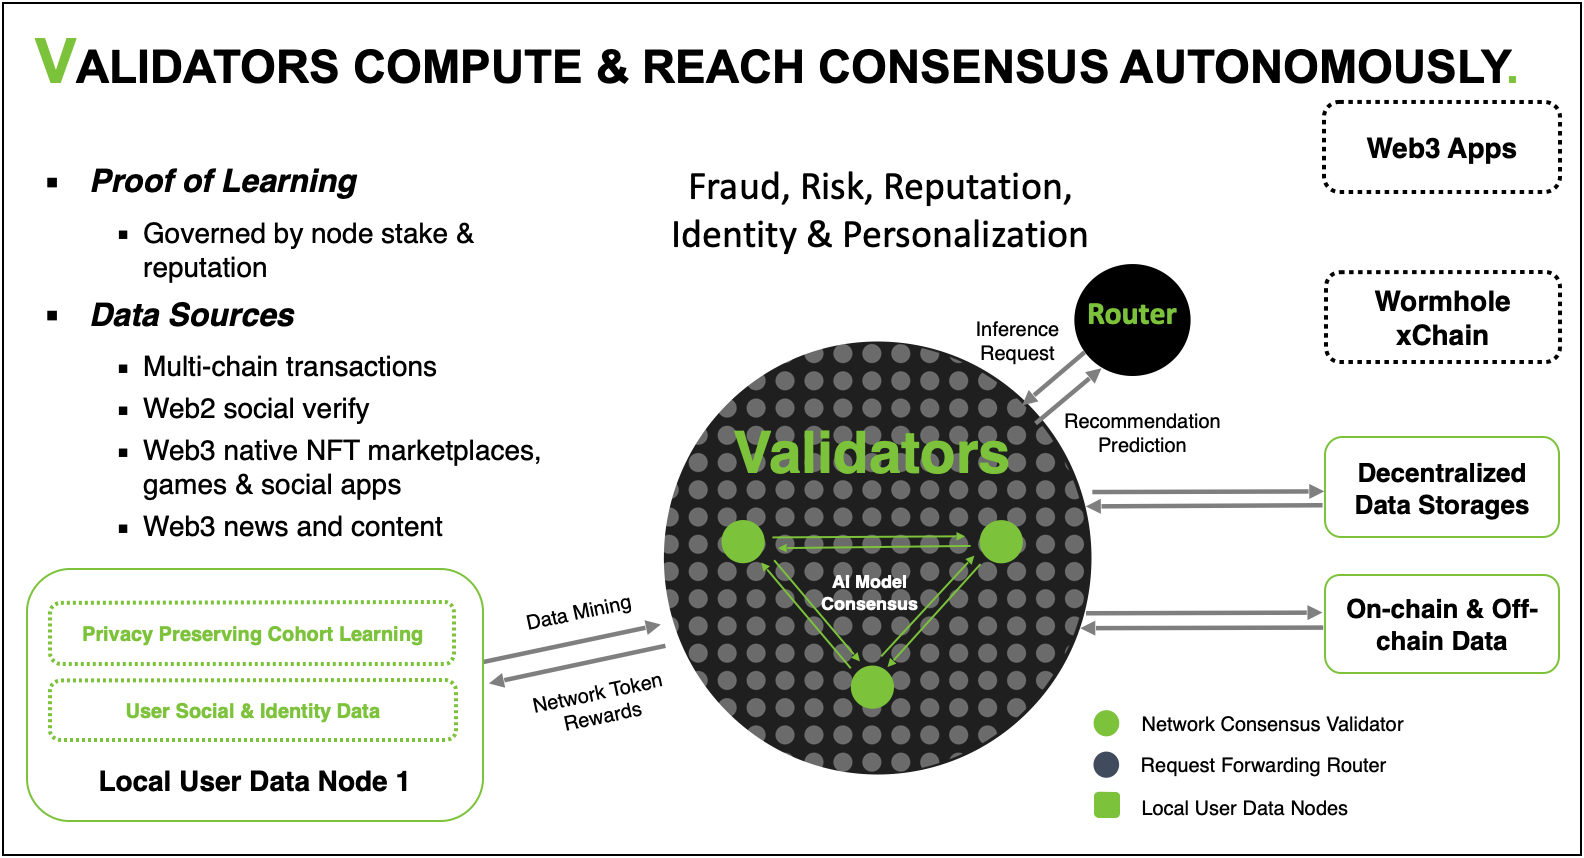
\includegraphics[width=6in]{fig/overall_arch.jpg}
\caption{BitNeuron Decentralized Network Architecture.} 
\label{fig:overall-arch}
\vspace{-2pt}
\end{figure}

\begin{figure}[t]
\centering
	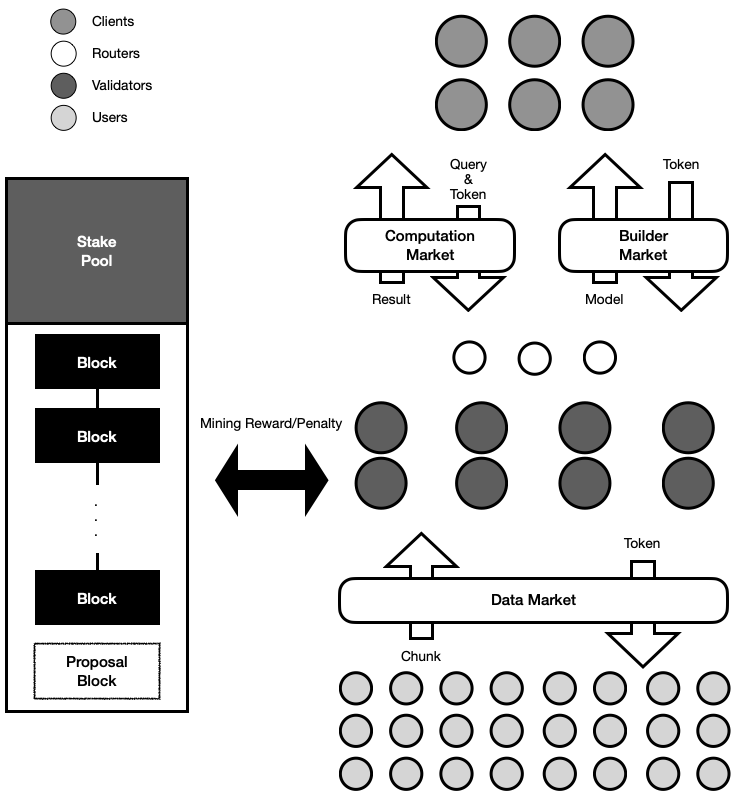
\includegraphics[width=0.8\textwidth]{fig/tokenomics.png}
\caption{BitNeuron Cycle.} 
\label{fig:tokenomics}
\vspace{-2pt}
\end{figure}

The key market participants in the network are:
\begin{itemize}
    \item \textbf{Users and Data Nodes.} Data nodes of the network represent users. Data nodes are incentivized by the network token rewards to propagate local data and models around the network in a privacy preserving manner. More specifically, they may participate in on-chain Data Market to broadcast encrypted data and model parameters to other nodes in exchange for BitNeuron tokens in a trustless manner. They are provers in the verifiable computaion with validators. In the following of the paper, Data Market and Local Model Market are used interchangeably because user data are represented as local models for privacy, and User and Data Node are used interchangeably because from the network perspective users are just data nodes.
    
    \item \textbf{Validators.} Validators maintain the blockchain through PoS with weighted voting. The nodes who deposit enough stakes in the network's stake pool can be the validators. The network prevents them from acting maliciously during the process by taking away the stakes of faulty nodes. They also act as data aggregation and model learning nodes. They process and learn data in a decentralized way via gossip learning protocol. Validators are verifiers of data node data for decentralization. Meanwhile, the models learned by each validator are verified with predefined evaluation metrics of each model. They have to prove to each other on the model learning results and model evaluation metric improvements. Reputations can be built for efficient validator discovery since they operate autonomously without centralized control to speed up the computations.
    
    \item \textbf{Clients and Builders.} Clients make data aggregation and model inference queries to the network. Those queries are answered by the validators with suitable data and model in a verifiable and tamper-proof way at the Compuatation Market. The clients who wish to go a step further and build their own model may build models for validators at the Builder Market. Builders can contribute models to the network by earning client BitNeuron token rewards. To focus the discussions on network operations, for simplicity, we do not differentiate clients and builders in the rest of the paper since they are both consumers of the infrastructure.
    
    \item \textbf{Routers}: Routers are the nodes who propagate and manage the orders from the clients. They match and verify the orders with some transaction fee incentives. They ensure trustless delivery of information to the clients. Therefore in BitNeuron, the clients can focus on building their applications. Routers only propagate the requests for BitNeuron token rewards, while the verifications and model validations are handled by validators.
\end{itemize}

In data-driven Web2 applications, data collection, storage, and learning is done by one central entity. Such system results in serious data privacy breaches. In order to resolve those issues, we replace the whole process by introducing three decentralized markets coordinated by multiple entities: Data Market (a.k.a., Local Model Market), Computation Market (a.k.a., App Query Market), and Builder Market. The supply and demand for data, models, and queries intersect at these markets. They are verifiable and tamper-proof information markets where the exchanges are made publicly through on-chain orderbooks: 
\begin{enumerate}
    \item Participants add offer (sell) and bid (buy) orders to the orderbook.
    \item When a pair gets matched, two parties add a deal order to the orderbook.
    \item The seller provides proofs for their service, and the proofs get verified.
    \item The buyer pays the seller, and the orders get cleared from the orderbook.
\end{enumerate}

The main driving force of the network tokens is the three markets. In these peer-to-peer algorithmic markets, the transactions, orders, and proofs that are involved in the trades should be submitted to the blockchain so that the trades can be verified by the validators. The participants get rewarded for the valid trades only, and this motivates the nodes to not act faulty.

\begin{itemize}
\item \textbf{Data Market.}
The users may participate in the Data Market if they decide to propagate their data pseudo-anonymously in exchange for the token rewards from the validators. They post the offer orders for their local data and model parameters, and once the orders get matched with bid orders, they get passed to the nodes with the matching orders in a privacy-preserving manner. The data and model parameters are backed by verifiable proofs to guarantee their integrity.

\item \textbf{Computation Market.}
There are two types of services provided by the validators to the clients at the Computation Market: data aggregation and model inference. The Computation Market is a decentralized alternative to the data servers of centralized platforms. It works like a job recruitment market; a client has a query (job) in mind and looks for the validators with data and/or model (caliber) that can answer its query. The routers guarantee that the results provided by the validators are trustworthy.

\item \textbf{Builder Market.}
The model builders contribute their expertise to the network and in turn collect a fraction of the network fees as rewards. The models are standardized with different prediction goals and validators select the best performing AI models, when fulfilling user queries.
\end{itemize}


As shown in  Fig.~\ref{fig:tokenomics}, BitNeuron blockchain record keeping is done by the validators. A validator may gain stake in BitNeuron by depositing BitNeuron tokens into stake pool. Its stake may get taken away if the node is involved in any malicious behaviors in the network such as not properly validating blocks, manipulating data, or faking query results. We also keep track of reputation scores for the validators, which is determined by the nodes' behaviors in the network. For example, a validator who purchased lots of data from Data Market, used them to train a model with high performance, and leveraged the data and the model to provide clients with query results will have a higher reputation score than a validator who did not participate in the markets often.

The blockchain is maintained via Proof of Stake (PoS) with weighted voting. At every epoch, a block proposer is elected pseudo-randomly from the validators in proportion to their stakes and reputation scores. The block proposer needs to create a new block and propose it. The proposal block is added to the network if the majority of the validators agree that the block is valid through a weighted voting, where the weights are determined by the nodes' stakes and reputation scores. Then, the block proposer gets rewarded for mining a new block.

\section{Privacy-Preserving and Decentralized Model Learning}

% \begin{figure}[t]
% \centering
% 	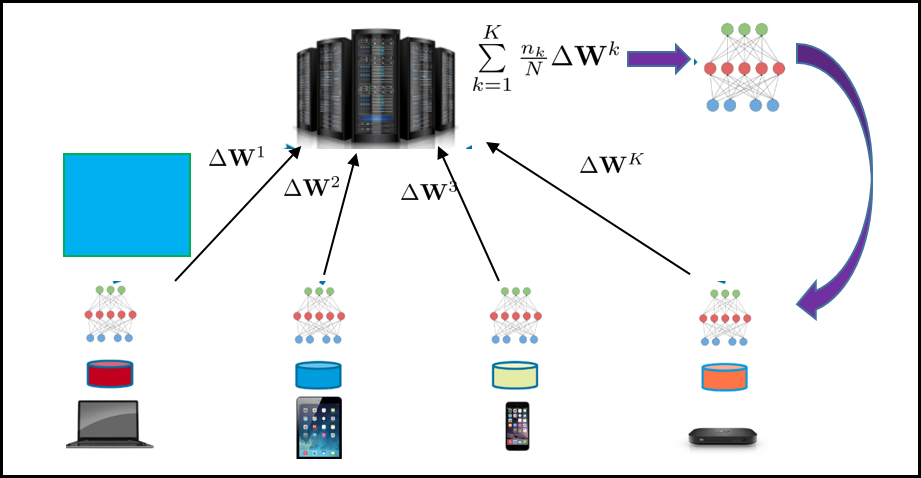
\includegraphics[width=6in]{fig/CT_FL.png}
% 	\caption{Federated Learning.} 
% \label{fig:FL}
% \vspace{-10pt}
% \end{figure}

Traditional machine learning techniques require the collection of local data to one centralized data server. In such centralized learning process:
\begin{enumerate}
  \item Local/personal data are transferred to a centralized server.
  \item The server performs learning on a master model.
  \item Model inference is controlled by the server.
\end{enumerate}
A Centralized learning framework, shown in Fig.~\ref{fig:FL} (a), does not have a native mechanism to ensure data privacy and security, and can easily collapse if the server is attacked or corrupted. Moreover, the revenues made from user data is not distributed to the users who actually own them. 

In partially decentralized learning approaches such as federated learning, the edge devices/nodes and a central server learn collaboratively without sharing local data as shown in Fig.~\ref{fig:FL}(b). The general process of federated learning is:
\begin{enumerate}
  \item Central server has a global model and local devices/nodes download the current global model.
  \item The local devices/nodes perform learning locally with their own data.
  \item The central server collects and summarizes the changes to update the global model.
  \item The new version of global model is pushed to every devices/nodes.
\end{enumerate}
Essentially, in decentralized learning, the central server's ability to learn and the need to collect user data are decoupled. In this way, the privacy of user data is preserved. Yet, the overall learning is still governed by one entity, which means that the whole network breaks when the server fails technologically or ethically. Moreover, the ownership of data is still not fully returned to their owners as there is no reward for the local nodes who helped the central server to learn with their local data and computing power. 

\begin{figure}[t]
\centering
	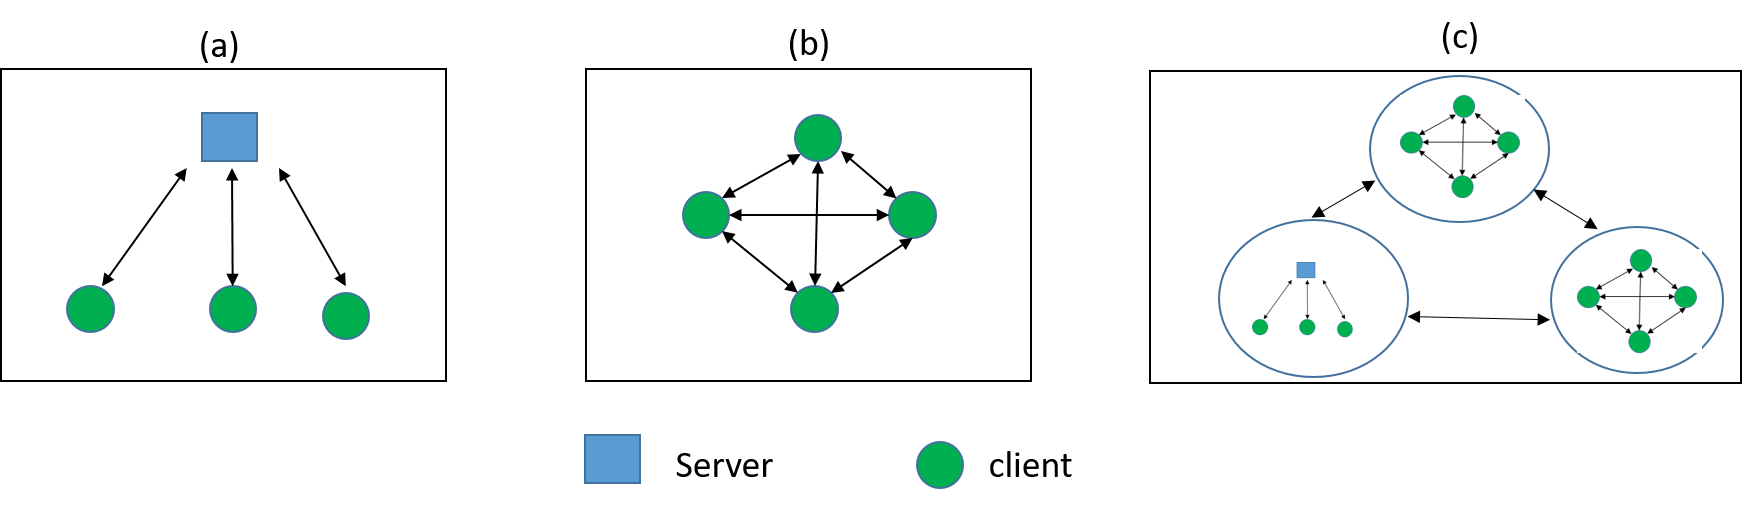
\includegraphics[width=6in]{fig/FL.png}
	\caption{(a) A centralized learning framework. (b) A partially decentralized learning framework. (c) A fully decentralized learning framework. } 
\label{fig:FL}
\vspace{3pt}
\end{figure}

\begin{algorithm}
\caption{Gossip Learning}\label{alg:gossip}
\begin{algorithmic}[1]
\State $w_k \gets$ init()
\Loop
    \State wait$(\Delta_g)$     \Comment{Wait for a time unit}
    \State $p \leftarrow$ select()   \Comment{Select a node}
    \State send compress$(w_k)$ to $p$
    \State $w_r \gets$ receive$()$  \Comment{Receive model from another node}
    \State $w_k \gets$ merge $(w_k,w_r)$
    \State $w_k \gets$ update$(w_k,D_k)$
\EndLoop
\end{algorithmic}
\end{algorithm}

The key idea behind protecting user data ownership and privacy is to adopt a fully decentralized learning method like gossip learning. In fully decentralized learning, the whole learning is coordinated by the local nodes without a central server orchestrating it as shown in Fig.~\ref{fig:FL} (c)~\cite{lalitha2018fully}. The pseudocode for gossip learning is shown in Alg.~\ref{alg:gossip}. In this framework, 
\begin{enumerate}
  \item A node $k$ initializes a local model $w_k$.
  \item Another node $p$ in the network is selected by a sampling service.
  \item Model parameter $w_k$ is compressed and sent to $p$. 
  \item It receives a model $w_r$.
  \item The node merges it with the local model $w_k$. 
  \item Then, updates $w_k$ using the local data set $D_k$.
\end{enumerate}
Merging is typically achieved by the weighted average of the model parameters. The most common update method is stochastic gradient decent (SGD).

\begin{algorithm}
\caption{Gossip Learning User $u$}\label{alg:gossip_client}
\begin{algorithmic}[1]
\State $\theta_u \gets$ init()
\Loop
    \State wait$(\Delta_g)$     \Comment{Wait for a time unit}
    \State $\theta_u$ = update$(D_u, \theta_u)$       \Comment{Update local model}
    \State $k_1,...,k_n \leftarrow$ selectValidators()   \Comment{Validators from Data Market}
    \State send encrypt$(D_u)$ to $k$
    \State send compress$(\theta_u)$ to $k$
\EndLoop
\end{algorithmic}
\end{algorithm}

\begin{algorithm}
\caption{Gossip Learning Validator $k$}\label{alg:gossip_validator}
\begin{algorithmic}[1]
\State $\theta_k \gets$ init()
\Loop
    \State wait$(\Delta_g)$     \Comment{Wait for a time unit}
    \State $D_r \gets$ receive$(D_{u_1},...,D_{u_n})$ \Comment{Receive data from users}
    \State $\theta_r \gets$ receive$(\theta_{u_1},...,\theta_{u_n})$ \Comment{Receive models from users}
    \State $D_k \gets$ merge$(D_k,D_r)$
    \State $\theta_k \gets$ merge$(\theta_k,\theta_r)$
    \State $\theta_k \gets$ update$(\theta_k,D_k)$
\EndLoop
\end{algorithmic}
\end{algorithm}

Our decentralized learning is based on the gossip learning. The users propagate their data and/or model parameters as described in Alg.~\ref{alg:gossip_client}, and the validators take the role of model learning as shown in Alg.~\ref{alg:gossip_validator}. In our fully decentralized learning,
\begin{enumerate}
  \item Users perform local learning with local data.
  \item Users offer their data $D_u$ and/or model parameters $\theta_u$ in Data Market.
  \item Encrypted data and compressed model parameters are transferred to the validators, who won the bid, in a privacy-preserving manner.
  \item In return, the users are rewarded with network tokens.
  \item The data and/or model parameters from the users are merged with the validators' local data $D_k$ and model parameters $\theta_k$.
  \item The validators update local models with the local data and model parameters.
  \item Validator nodes with enough stakes and reputation scores validate 1 - 6 and get rewarded with network tokens.
\end{enumerate}
For decentralized learning in a trustless network, we need a consensus mechanism to deal with malicious and dishonest nodes who want to corrupt the learning.

\section{Proof of Gradient - Model Learning \& Inference Consensus}

\begin{figure}[t]
\centering
	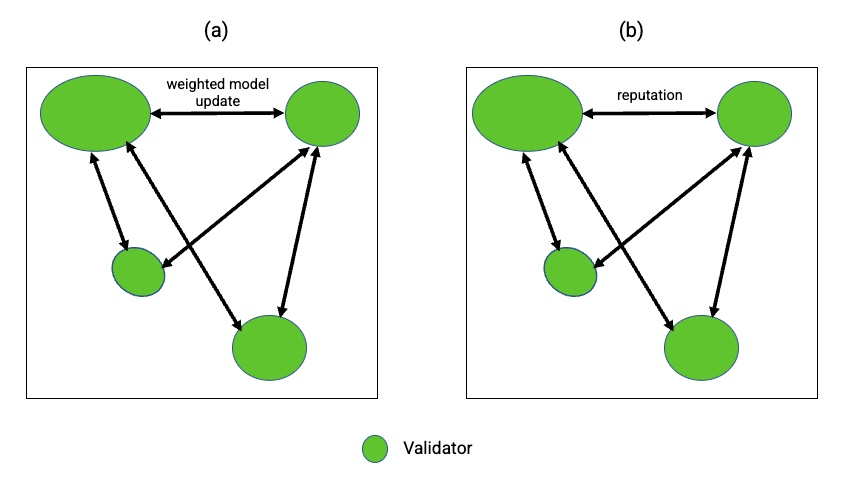
\includegraphics[width=0.9\textwidth]{fig/consensus.jpg}
\caption{Weighted voting with the Proof-of-Stake.} 
\label{fig:voting}
%\vspace{-10pt}
\end{figure}

The PoS with weighted voting is employed as a consensus mechanism in BitNeuron. Compared to simple majority voting, weighted majority voting is more immune to Sybil attacks where an attacker creates and controls multiple nodes and manipulates the voting. If the voting is weighted by the amount of stake that each validator has, it is much more difficult to execute a Sybil attack because the attacker has to spend significant amount of resources to gain high stake in the network as demonstrated in Fig.~\ref{fig:voting}.

The network robustness comes from the fact that the nodes with bad behaviors such as tampering data and forging model updates and/or inference can be penalized by taking away their stakes, making them suffer economically. To be extra safe, reputation scores, which reflect validators' data storage, model performance metrics, and past interactions with other nodes in the network, will be considered in the weighted voting.

During data learning, the validators performing the learning through the merge and update functions from Alg.~\ref{alg:gossip_validator} need to provide proper proofs that they are not forging the process. Otherwise, their model training will not be approved by the network. Likewise for model inference, the validators need to prove that their query results are valid. Not doing so will cause their stakes and reputation scores to be reduced.

Under this mechanism, the speed of validating a new block will dictate how fast the models learn and predict. Therefore, we may accelerate the voting process by putting a threshold on the stakes and reputation scores for deciding which nodes can participate in the voting.

\section{Handling Corrupted and Faked Data.}
Different methods will be implemented to handle corrupted and faked data:
\begin{itemize}
    \item Corrupted data samples are from valid users, but the data may miss partial information. We want the learning models still work for this kind of corrupted data. Therefore, data corruptions will be considered in the training process via adversarial training or distributionally robust training~\cite{sattler2019robust}. The robustness against corrupted data samples can be further improved by implementing a simplified version of the self-healing method~\cite{chen2022self}. In practice, many data corruptions are unpredictable, so even a model from robust training may still not work well. Instead, we can add some plug-in blocks to the trained model, such that the errors can be identified and mitigated in the prediction process. Specifically, a low-dimensional manifold could be learnt to characterize the ``good" behavior of every layer, and the undesired features outside of the manifold can be removed in the forward propagation to avoid or mitigate prediction errors.
    
    \item Faked data samples are unwanted in the learning: including them in the learning process can produce a model that provides wrong prediction results. To handle faked data, we will implement a data selection process~\cite{roh2021sample} based on two criteria. Firstly, before the model is re-trained, we only select data samples that have low loss function to participate in the training. This will prevent faked data to cause degraded prediction performance. Secondly, we will set an upper bound for the number of samples selected from each group. This will prevent system collapse caused by the infinite faked data produced in the network. 
\end{itemize}


\section{Improving Communication Efficiency via Compressed Learning}

A fundamental challenge of a decentralized learning framework is how to handle the huge communication cost caused by the large model size. This challenge will be solved efficiently via compressed training~\cite{hawkins2022towards,hawkins2021bayesian} in our framework. Specifically, we will implement tensor-compressed training, which has achieved the best compression so far in the training process.
\begin{figure}[t]
\centering
	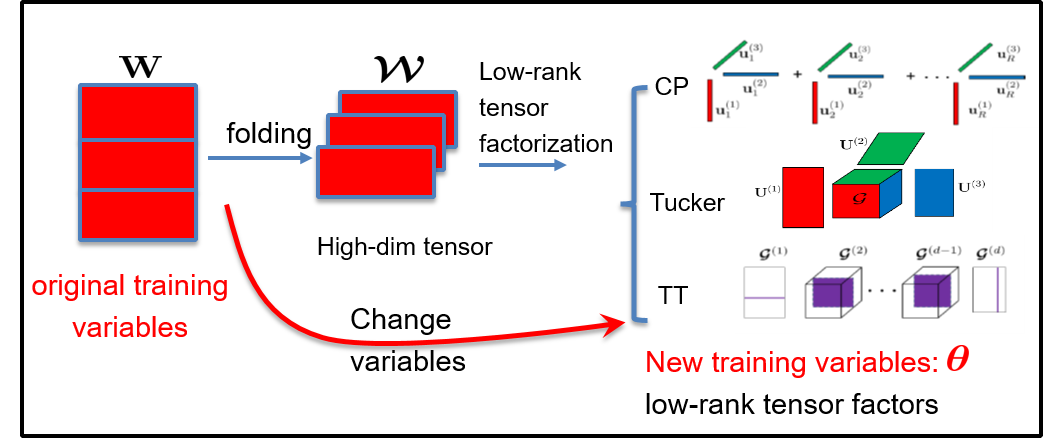
\includegraphics[width=6in]{fig/tensor_compression.png}
\caption{Reducing model parameters by compressing training variables via low-rank tensor factorization. } 
\label{fig:aws_overview}
%\vspace{-10pt}
\end{figure}

\begin{figure}[t]
\centering
	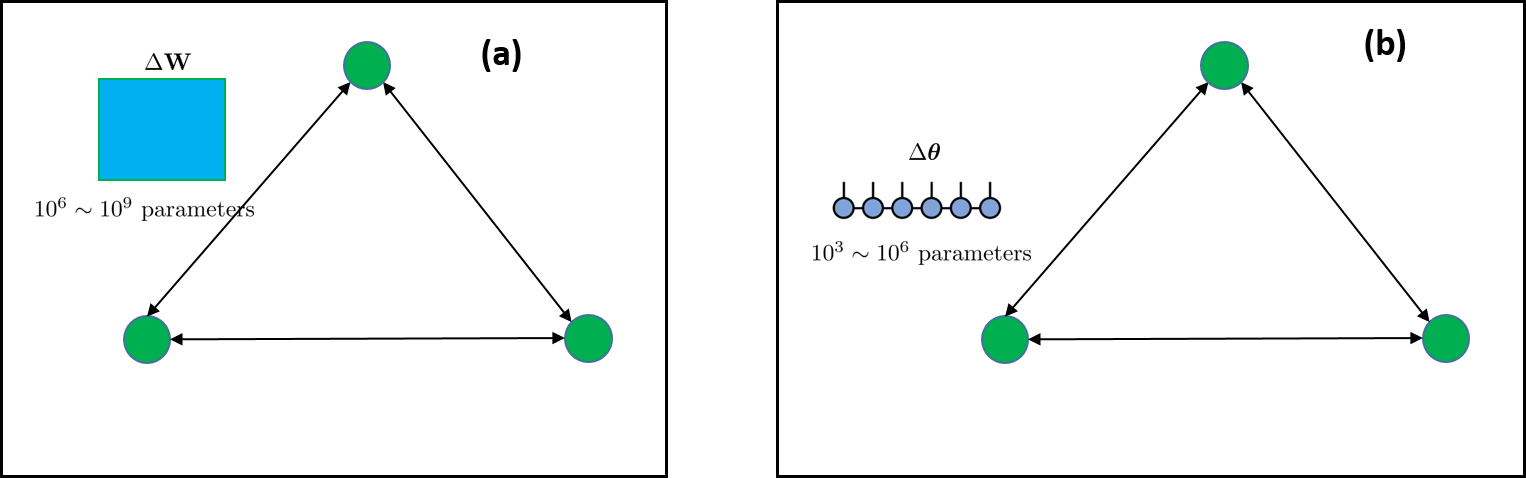
\includegraphics[width=6in]{fig/TT_FL.png}
\caption{(a) A conventional decentralized learning method needs to share the full-size model information. (b) In our proposed tensor-compressed decentralized learning method, we only share the compressed tensor factors to save the communication cost. } 
\label{fig:TT_FL}
\vspace{-10pt}
\end{figure}

\paragraph{Low-rank Tensor-Compressed Training.} As shown in Fig.~\ref{fig:aws_overview}, the model parameters (such as weight matrices and embedding tables) of recommendation systems have lots of redundancy. Because of such redundancy, low-rank approximation can be used to approximate the original model parameters with orders-of-magnitude less model parameters. In the training process, the original 2-D or 3-D model parameters $\mat{W}$ will be folded into high-dimensional data arrays (e.g., tensors). Each tensor can be represented with some low-rank factors $\boldsymbol{\theta}$ in a specific compact tensor decomposition format. In the training process, we only need to compute $\boldsymbol{\theta}$ instead of $\mat{W}$. As illustrated in Fig.~\ref{fig:TT_FL}, typically $\boldsymbol{\theta}$ has $10^3 \times 10^5$ variables while $\mat{W}$ has $10^6 \sim 10^9$ variables, so thousands of times of compression can be achieved on large recommendation system models~\cite{hawkins2022towards}. 

\paragraph{Communication Cost Reduction.} To address the communication bottleneck of decentralized learning, only $\boldsymbol{\theta}$ needs to be transferred as shown in Fig.~\ref{fig:TT_FL}, so the latency caused by network communication can also be reduced significantly. Low-precision and mixed-precision representations can also be used to represent the compressed parameters, which can further reduce the communication cost. The key idea is to use a small number of binary bits to represent all variables in the tensor factors. Promising numerical results and hardware demo have been reported in~\cite{yang2022hardware,zhang2021fpga}. Such low-precision representation will greatly save the computing, memory and communication cost in federated learning, but it will not cause significant loss of prediction accuracy due to the error-resilient nature of neural networks. The compressed model parameters can be stored on local devices with small memory cost to enable fast inference. 

\section{Decentralized Data Aggregation and Analytics}

Data aggregation is the process where raw data collected from multiple sources are processed and presented in summary statistics such as average, sum, and count for statistical analysis. For example, we can gather information about NFT transactions for a certain period of time and provide observations such as:
\begin{itemize}
    \item Average, minimum, and maximum price in 24 hours.
    \item The average frequency of transaction by NFT.
    \item The number of buyers by NFT collection.
\end{itemize}
In other words, a data aggregation tool enable its users to ask questions (queries) and get answers (responses) from large amount of data. 

The most widely used programming language for data management is Structured Query Language (SQL). SQL can be used to query, manipulate (insert, update, and delete), define, and access data. Its keywords such as GROUP BY, MIN, MAX, COUNT, AVG, and SUM let us easily get summarized statistics from raw data.

As illustrated in Fig.~\ref{fig:overall-arch}, DApps built on top of BitNeuron can use usual SQL queries to get the on-chain data analytics with some transaction fee. Once a query is made by the application, the query will be posted to the Computation Market orderbook, and the routers may propagate the order around the network. Then, the validators with proper data will process the data and respond to the query. Usually a central database is involved in many decentralized data solutions due to the low speed of blockchains. In BitNeuron, we can use varying stake and reputation score thresholds to speed up the data aggregation process. In this way, BitNeuron can respond to large enterprise scale data requests without moving the data off-chain.

Moreover, BitNeuron supports extract, transform, and load (ETL) pipeline.  Both batch ETL, where data is accumulated and processed in batches during a batch window, and online ETL, where data is processed as soon as it arrives, are supported. Batch ETL is useful for dApps that want to be cost-effective and need to process large volumes of data. On the other hand, online ETL can help dApps that have delay sensitive functionalities such as fraud detection. Since BitNeuron has both batch and online ETL functionalities, it can be used for both online analytical processing (OLAP) and online transaction processing (OLTP).

As mentioned above, BitNeuron data consensus mechanism is PoS with weighted voting. As in model learning and inference, the validators participate in verifying data collection and processing on-chain. A node that performs data aggregation needs to generate and submit the proofs. Failing to do so will result in losing their stakes. In addition, stake and reputation score threshold is actively managed in order to respond to different types of queries made by dApps. For the queries that are complex and require lots of data, we will lower the entry threshold so that many validators can participate. On the other hand, the queries that are simple and focus on short atomic data can be managed by fewer validators by raising the threshold.

\section{Applications}
BitNeuron is to enable the next generation DApps. Ecosystem applications include but not limited to:
\begin{itemize}
    \item Wallet and protocol forensics for identity, security and fraud detection.
    \item "Smarter" protocols such as more complex autonomous market makers (AMMs) and lending protocols that are driven by real-time data about wallets, users and contracts.
    \item Safer protocols with fraud, anomaly, and network intrusion detection.
    \item Data-driven DeFi and NFT trading.
    \item Web3 protocols that require user data such as identity, reputation, social behavior, and recommendation protocols.
    \item Web3 native social networks like LinkedIn, Facebook, TikTok, Instagram and so on while preserving user data privacy and ownership.
    \item Data-driven investment, grants, and social decentralized autonomous organizations (DAOs) that run based on data analytics.
    \item Chain agnostic identity system leveraging offchain and onchain user data.
\end{itemize}

\section{Token Distribution and Governance}
There are $10,000,000,000$ network tokens and this total supply will not increase. Furthermore, all the tokens are contractually locked and released following the token
distribution design. The network is fully governed by BitNeuron token holders with governance proposals and voting mechanisms, though the governance mechanism will be fully disclosed once the network is online and through network participant voting. the supply of both locked and unlocked tokens will be allocated according to Table \ref{table:token-distribution}.

\begin{table}[h!]
  \begin{center}
    \begin{tabular}{l S S l}
      \toprule % <-- Toprule here
      \textbf{Purpose} & \textbf{Release Schedule} & \textbf{Total} \\
      \midrule % <-- Midrule here
      Network Rewards & Unlock over 7 years with an initial 1-year cliff & $20\%$\\
      Team Members & Unlock over 4 years with an initial 1-year cliff & $20\%$\\
      Partners $\&$ Advisors & Unlock over 4 years with an initial 1-year cliff & $5\%$ \\
      Private Sale  & Unlock over 4 years with an initial 1-year cliff & $20\%$ \\
      Ecosystem Participation  & Unlock over 4 years with an initial 1-year cliff & $35\%$ \\
      \bottomrule % <-- Bottomrule here
    \end{tabular}
  \end{center}
  \caption{Allocation of the network tokens. The network rewards decrease over time.}
    \label{table:token-distribution}
\end{table}





\section{Related Work}
This section discusses the evolution of decentralization technologies and Web2 data intelligence. 

\subsection{Bitcoin}
In the evolution of blockchain, Bitcoin was the first viable solution for internet money and decentralized network. After that, numerous coins and blockchains were built. Among them, Ethereum improved decentralization and pioneered smart contract platform to build the Web3 infrastructure. In recent few years, combined with Proof of Stake, initially proposed by PeerCoin, building scalable Web3 smart contract platform has been the focus.

Bitcoin is a decentralized digital currency that can be transferred on the decentralized bitcoin network. The peer-to-peer network of nodes running bitcoin software maintain the bitcoin blockchain which is a public records of bitcoin transactions. The network nodes independently store a copy of the blockchain and validate transactions and append them to their own copies of the blockchain and transmit the additions to other nodes. In every epoch, a new block that contains a new batch of valid transaction records is added to the block chain and issued to all nodes. The record keeping of the blockchain is done by the miner nodes by using their computer processing power. The easy to verify but hard to solve proof-of-work (PoW) is required in each new block to be accepted by the rest of the network. More specifically, Merkel Trees are adopted so that the non-miners can use the block header to verify a new blockchain without checking all past transactions. Once a new block is accepted by the rest of the network, the  miner who successfully solved the problem is rewarded with newly created bitcoins and transaction fees.

\subsection{Ethereum}

Ethereum inherits Bitcoin ecosystem's consensus, decentralization, and cryptography. While Bitcoin is limited as a simple ledger, Ethereum blockchain has a built-in Turing-complete programming language that allows anyone to write smart contracts and develop decentralized applications (dApps) on top of it. Ether (ETH) is the native cryptocurrency of Ethereum blockchain that is paid to the miners as transaction fees. Due to their autonomous nature under their own logic, Ethereum contracts are often called smart contracts. The codes in the contracts are written in Ethereum virtual machine (EVM) code, a low-level, stack-based bytecode language. The EVM is the runtime environment of Ethereum that includes a stack, memory, gas balance, program counter, and the persistent storage for all accounts. When a transaction calls a contract's function, the EVM translates and executes the contract's code into stack operations. A transaction sender must pay the miner, who is running the EVM and adding the transaction to the blockchain, a certain amount of gas fee in ETH. The gas fee system can reduce the amount spam transactions.

\subsection{Proof-of-Stake}
During "the Merge", Ethereum switched its consensus mechanism from Proof-of-Work to Proof-of-Stake. PoW has a scalablitiy issue because it requires more computer processing power as networks grow and wastes a lot of energy. PoW's security in trustless networks comes from the miners who are competing to be the first one to solve the puzzle; therefore as more miners join the network, its security increases. On the other hand, PoS is more scalable and suitable for blockchains like Ethereum that not only serves as a ledger but also as an infrastructure for dApps, and need to not only process incoming and outgoing ETH transaction but also has to process transactions from decentralized finance (DeFi), non-fungible token (NFT) minting and sales, and more. In PoS, a blockchain employs a network of validators who stake their own tokens into a pool to get a chance to validate new transactions, update the blockchain, and get rewarded. A majority consensus has to be reached in order for a block to be accepted and added to the blockchain. Weighted voting can be adopted to improve the robustness of the consensus, where the weight is determined by the node's profile such as the amount of stake and reputation.

\subsection{Fully Decentralized Learning}
In contrast to traditional machine learning techniques where all local data stored at local nodes are uploaded to a centralized server, decentralized learning like federated learning and gossip learning enables the client data to be only kept on local devices/nodes without being shared in the network. Generally in federated learning, local models are trained with local data and the model parameters are exchanged at some frequency to learn a global model that is shared by all nodes. Under such set up, a central server orchestrates the learning process. The central server initializes a global model and broadcasts it to the network and then individual nodes will train the model with local data. Once the local training is complete, the central server collects the training results from the nodes and updates the global model with some rule (generally averaging) which is again transferred to every nodes. On the other hand, in fully decentralized learning, such as gossip learning, there is no central server and the nodes themselves coordinate the learning.

\subsection{Low-rank Tensor Compressed Training}
A tensor is a multi-dimensional collection of numbers that can be thought of as a matrix extended to higher dimensions than 2-D. The motivation behind tensor decomposition comes from matrix factor analysis, which breaks down a matrix into two factors that contain latent relationships. Low-rank tensor decomposition can compress a large tensor while retaining the latent information inside it. Therefore, it has been one of the most effective approaches to reduce the memory and the computational costs of neural networks. In general, the model parameters are compressed after the training to reduce storage requirement and shorten inference time. However such methods cannot benefit from the reduced memory during training. Instead by using an end-to-end low-rank tensor compressed training algorithm, the advantage of compression can be enjoyed during training time, and the model can be optimized for the compressed setting.

\subsection{Mixed-precision Training}
Mixed-precision utilizes numerical formats with lower precision than 32-bit floating point which is a mainstream numerical format used to represent model parameters in machine learning. Lower precision numbers translate to less memory and faster mathematical operations. As a result models trained with mixed-precision training algorithms require less memory to be stored, and their training and inference time gets shortened. Such benefits come without losing any task-specific accuracy compared to the full precision training by identifying the parameters that require full precision (i.e., 32-bit floating point) and adopting lower precision representation to the parameters that can be represented with lower precision. 

\subsection{Personalized Recommendation}
Deep learning is widely adopted to achieve personalized recommendations for search, social apps, and user interest discovery. In particular, the state of art is to build a user side deep learning model (a.k.a., user tower) and an item side deep learning model (a.k.a, item tower), together with a ranking model to combine them for final predictions \cite{DLRM19,ArchImpl19,QuoRemTrick19}. The model parameter size can be hundreds of Gigabytes or even Terabytes. Recommendation models are the key driver and brain of the mainstream Web2 applications. A Web3 data intelligence infrastructure is needed to support such model computations and real-time predictions to indeed decentralize data ownerships.

\subsection{Identity, Targeted User Growth, Fraud Detection and Risk Management}
Together with personalized recommendation, identity, fraud detection and risk management form the key data intelligence solutions powering the current Web2 data and social applications. The blockchain and crypto data are nothing different from Web2 with a) onchain transaction data similar to credit card transaction data in Uber, Doordash, Airbnb and Instacart, b) offchain data including image (e.g., NFTs), natrual languages, and metadata, and c) biometrics data including wallet fingerprints, location, and account verifications \cite{uberfrauddetection,uberhumaninloop,ubermastermind}. A Web3 data infrastructure is missing to get access to such data and build similar technologies for a more secure, identifiable and privacy preserving Web3 world.

\subsection{Web3 Analytics, Security LoopHoles and SocialFi}
While delivering a lot of value to the world with censorship resistant, Web3 identity and social solutions, the Web3 community is still building very naive solutions from the data intelligence perspective. For example, the mainstream analytics tools (e.g., Nansen) only support very simple analysis, which are solutions long deprecated by Web2 data community. Most of security, fraud, and financial crime issues can be easily detected with intelligent solutions like machine learning and data clustering by using public data only. With emergence of Web3 social, metaverse and games, how to leverage Web2 data intelligence technologies such as personalization, fraud detection, identity and risk management is critical to their success and user data decentralization.

\section{Conclusion}
In this paper, we have proposed an ultimate Web3 data intelligence infrastructure that is scalable and with data learning and aggregation capacity. Many Web3 solutions out there are not as decentralized as they seem. This is mainly because most popular blockchain applications still use the centralized server system to store user data and provide services around them. On the other hand, the BitNeuron deals with user data in a fully decentralized manner and can serve the requests made by applications without relying on a centralized backend server. In addition, the transaction fees collected during model inference and data aggregation are naturally circulated around the network, not only to the validators but also to normal users, through the market system. In this way, BitNeuron can be a solution to returning data and network ownership to the users. BitNeuron is also client-friendly as we may adjust the the stake and reputation score thresholds for the weighted voting with PoS to speed up the serving time for the requests made by the clients. Therefore, Web3 native data-driven applications can be built on top of it in a truly decentralized way.

\bibliographystyle{IEEEtran}
\bibliography{Bibliography}

\end{document}
